\documentclass[twoside,project,skipblank]{../MFFPrace}
\usepackage{pdfpages}
\usepackage{pdflscape}
\usepackage{multirow}
\usepackage{array}


\NazevPrace{Chromatická holografie\\\Large{Dokumentace elektronické části}}
\AutorPrace{Michal Ciesla}
\RokOdevzdani{2023}
\Katedra{Katedra chemické fyziky a optiky}
\Vedouci{RNDr.~Eva~Schmoranzerová,~PhD.}

\begin{document}
\maketitle
\begingroup
\let\clearpage\relax
\tableofcontents
\listoffigures
\listoftables
\endgroup
\appendix
\setcounter{chapter}{2}
\chapter{Dokumentace elektronické části}

\section{Úvod}

\section{Schéma}
Obvod je ve schématu na stránce \pageref{fig:schema} rozdělen do 6 logických částí:
\begin{itemize}
    \item \textbf{\textsf{Mode Select}}: Dvoustavový přepínač režimu fungování systému
    \item \textbf{\textsf{Status}}: Indikační RGB LED ukazující stav systému\footnote[1]{V průběhu expozice jsou indinkační diody vypnuté.} (červená = chyba, modrá = manuální režim, zelená = automatický režim)
    \item \textbf{\textsf{Manual Color Select}}: Tlačítko pro nastavení barvy a zastavení expozice, tlačítko pro zapnutí dosvětlovací LED a spuštění expozice, trojice barevných LED odpovídajících barvám laserů indikující jejich zapnutí\footnotemark[1] v manuálním režimu a dvojice LED indikující stav dosvětlovací LED a externího laseru\footnotemark[1]
    \item \textbf{\textsf{TTL}}: Výstup signálu do externího laseru
    \item \textbf{\textsf{Lasers}}: Lasery a jejich řízení a napájení
    \item \textbf{\textsf{Finishing LED}}: Dosvětlovací LED a její řízení a napájení
\end{itemize}
Mimo tyto logické části se dále nachází:
\begin{itemize}
    \item $9\:\text{V}$ stejnosměrný zdroj s vyhlazovacím kondenzátorem
    \item Bzučák
    \item Mikrokontroler \textit{Raspberry Pi Pico}
\end{itemize}

\begin{landscape}
    \centering
    \begin{figure}
        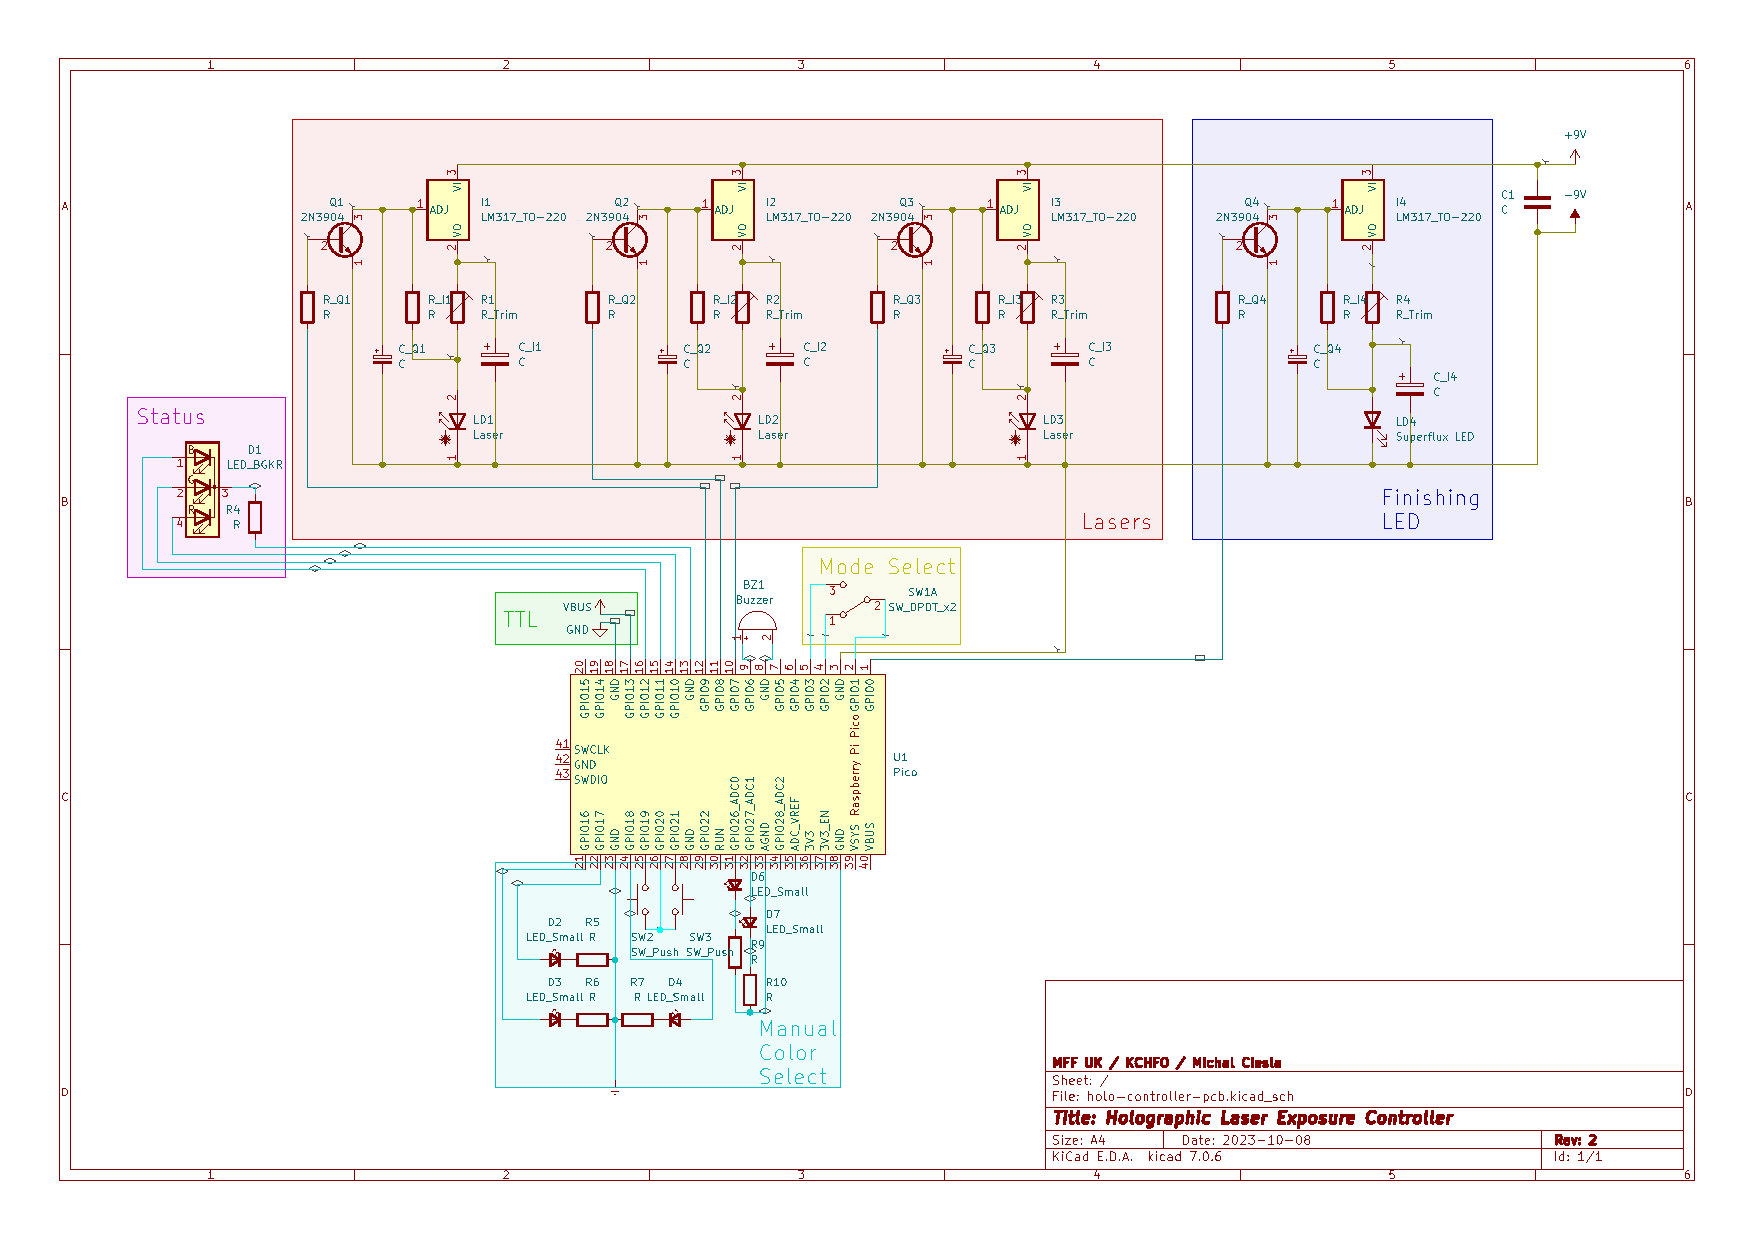
\includegraphics[width=19.3cm]{../../HoloControl-PCB/holo-controller-schema.pdf}
        \caption{Schématický návrh elektronického obvodu}
        \label{fig:schema}
    \end{figure}
\end{landscape}

Napájení laserů a dosvětlovací LED je realizováno regulátory napětí \textit{LM317T} v zapojení proudového stabilizátoru (převzato z \url{https://forum.arduino.cc/t//99890/8}). Aby bylo dosaženo potřebných proudů, jsou části \textsf{Lasers} a \textsf{Finishing LED} napájeny externím $9\:\text{V}$ stejnosměrným zdrojem. $9\:\text{V}$ spoje jsou na schématu vyznačeny žlutě.

Zbytek obvodu je napájen skrze \textit{Raspberry Pi Pico}, která samotné je napájeno pomocí USB ($5\:\text{V}$) z počítače či tabletu používaného pro ovládání. $5\:\text{V}$ spoje jsou na schématu vyznačeny tyrkysově.

$5\:\text{V}$ část a $9\:\text{V}$ část mají sdílenou zemi, spojení se nachází na pinu 3 mikrokontroleru.

\section{Plošný spoj}
Deska plošného spoje, vykreslená na obr. \ref{fig:pcb}, se skládá ze třech částí: hlavní řídící desky, desky pro ovládací prvky a desky pro dosvětlovací LED. Vyrobenou desku je nutné na tyto tři části rozdělit -- efektivním postupem je odlamovacím nožem naříznout desku podél natištěných čar a následně obyčejnými nůžkami desku rozstřihnout.

\medskip

Deska plošného spoje byla vyrobena firmou \textit{JLCPCB}.
\subsection{Poznámky k osazení desky}
Deska a součástky jsou navrženy pro THT pájení. Doporučujeme si připlatit za kvalitní cínovou pájku, opravdu to stojí za to \texttt{:)}.

\subsubsection{Mikrokontroler}
Pozice mikrokontroleru je vhodné nejprve osadit nožovými konektory pro možnost rychlé výměny mikrokontroleru. Zároveň se tím vyhneme poškozením mikrokontroleru teplem při přímém pájení.


\begin{landscape}
    \centering
    \begin{figure}
        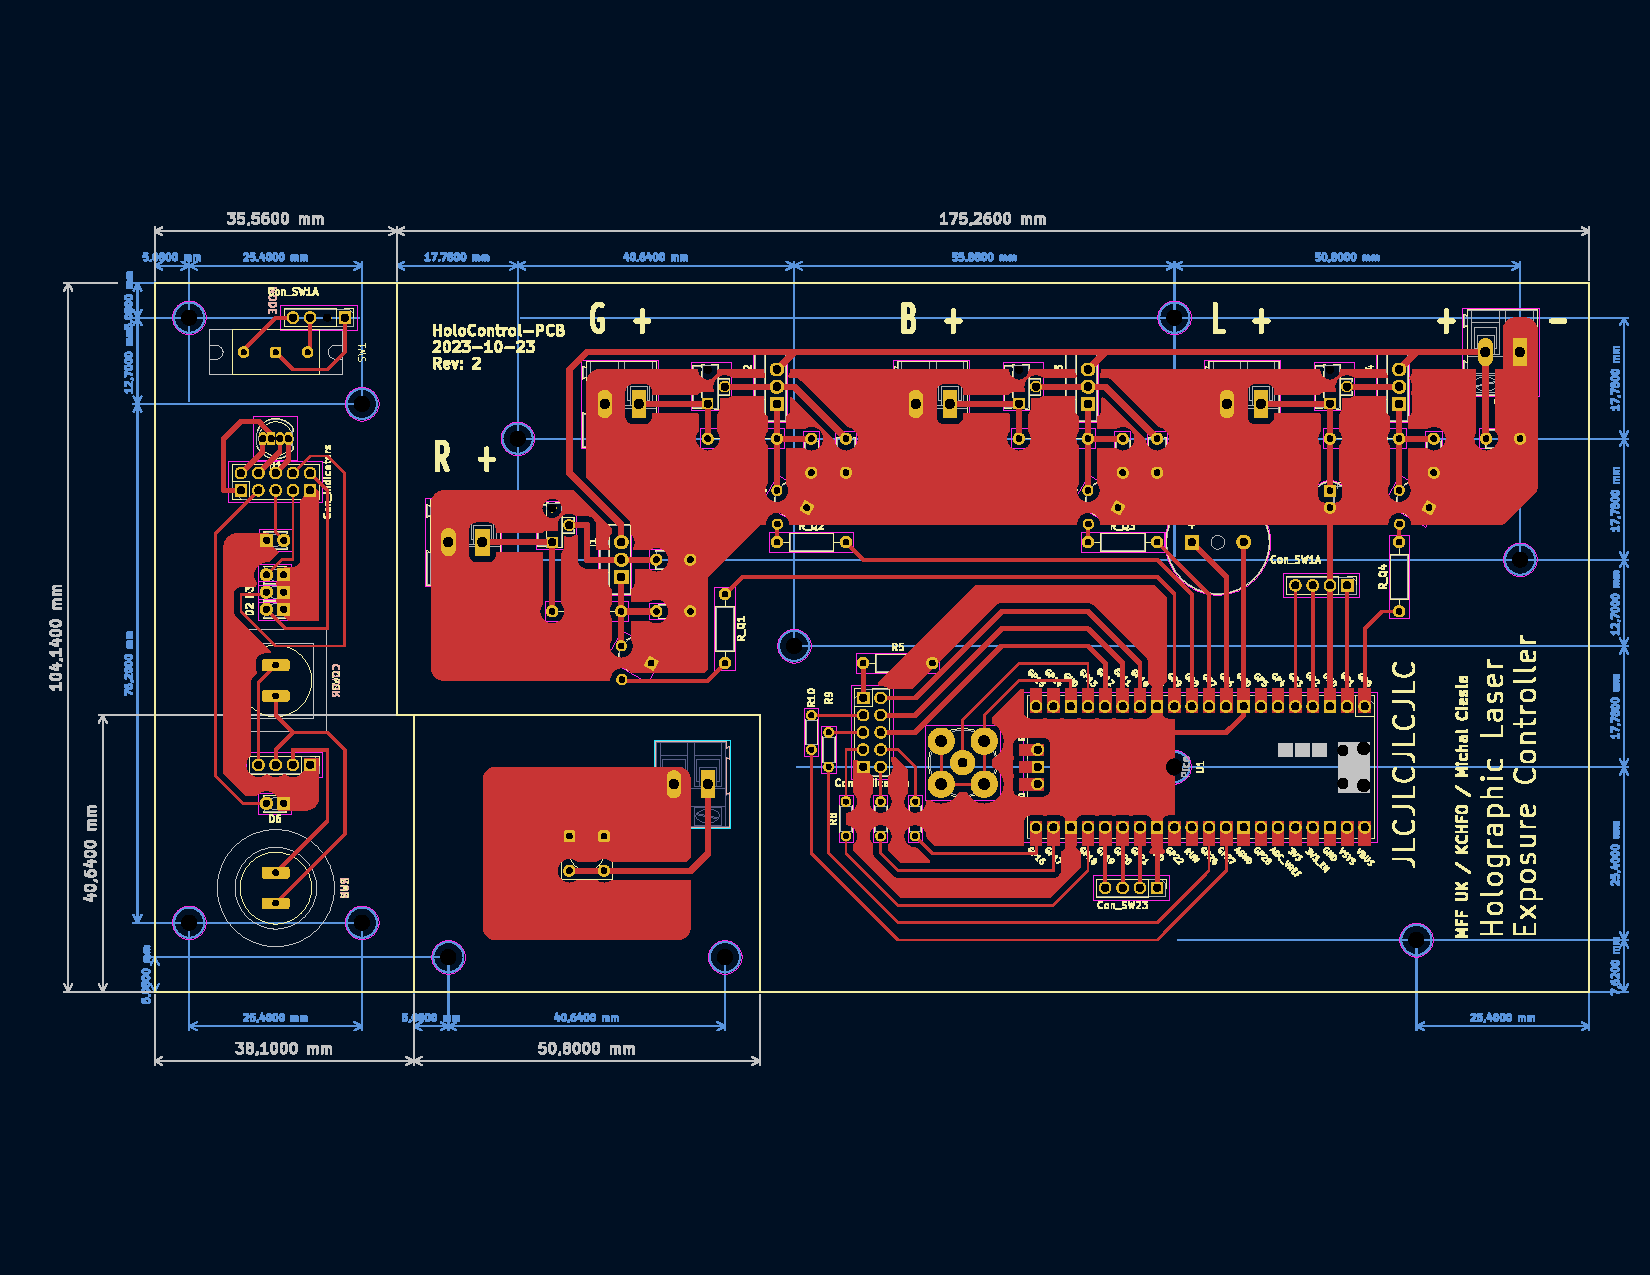
\includegraphics[width=19.3cm]{../../HoloControl-PCB/holo-controller-pcb.pdf}
        \caption{Deska plošného spoje v digitálním formátu s kótami}
        \label{fig:pcb}
    \end{figure}
\end{landscape}

\subsubsection{Napájecí obvody laserů a dosvětlovací LED}
Napájení laserů a superflux LED je zajištěno zapojením založeným na lineárním stabilizátoru napětí \textit{LM317T}, který pomocí zpětné vazby bude udržovat konstantní proud a lze jej vypínat přilehlým tranzistorem.

Velikost proudu se nastavuje trimrem u každého ze stabilizátorů. Nejbezpečnějším způsobem nastavení proudu je plně osadit hlavní desku plošného spoje, připojit $9\:\text{V}$ zdroje, poté zapojit multimetr či ampérmetr do svorkovnice u příslušného stabilizátoru "`nakrátko"' a šroubovákem nastavit trimr tak, aby měřící přístroj ukazoval vhodný proud pro laser nebo diodu, které budou na dané svorkovnici připojené.

Pozor, chladič na pouzdře stabilizátoru je přímo spojen s jednou z nožiček, takže se při pájení zahřívá a není příjemné za něj součástku držet.

\subsubsection{Ovládací panel}
Na ovládací panel se osazují jen konektory (ze zadní strany) a LED (z přední strany). U konektorů je důležité dodržet orientaci, aby ovládací panel spojovaly správně s hlavní deskou. Toto je důležité hlídat i při montáži konektorů na kabel.

Tlačíka i přepínač se musejí nejprve namontovat do ovládací krabice. Jsou ale vybaveny pájecími oky, vhodným postupem je proto umístit kousky drátů do pájecích ok a trochou cínu je upevnit, namontovat tlačítka a přepínač do ovládací krabice, upevnit plošný spoj ovládacího panelu do příslušné části ovládací krabice a poté mechanické spojení obou dílu krabice a připájení drátů do plošného spoje.

Tento proces je velmi složitý na jemnou motoriku a ovládání páječky, vybavte se proto notnou dávkou trpělivosti \texttt{:(}.

\subsubsection{Dosvětlovací LED}
Dosvětlovací LED se pájí z přední strany desky plošného spoje, svorkovnice ze zadní. Stojánek na dosvětlovací LED je navržen tak, aby do něj plošný spoj šel umístit osazený. Hlídejte si však orientaci svorkovnice, aby kabel po umístění do stojánku směřoval dolů.

\section{Ovládací krabice, stojánek}

\section{Seznamy použitých součástek}
\subsection{Elektronické součástky}
\begin{landscape}
    \catcode`\-=12
    \begin{table}[!h]
        \centering
        \caption{Seznam aktivních a pasivních elektronických součástek}
        \begin{tabular}{|l|l||c|l|r||l|l|l|l|}
            \hline
            \multicolumn{2}{|l||}{\textbf{Specifikace}}                                  & \textbf{Kód}                                   & \textbf{Úplná specifikace}                       & \textbf{Počet}                                           & \multicolumn{4}{l|}{\textbf{Pozice}}                                                                                          \\\hline
            \multirow{4}{*}{Rezistor}                                                    & $1\text{k}\;0{,}6\:\text{W}$                   & \texttt{110-073}                                 & \tiny{GYM/CYM RM 1k 0,6W 1\% 0207}                       & 4                                    & \texttt{R\_I1}        & \texttt{R\_I2}        & \texttt{R\_I3}        & \texttt{R\_I4} \\\cline{2-9}
                                                                                         & \multirow{2}{*}{$4\text{k}7\;0{,}6\:\text{W}$} & \multirow{2}{*}{\texttt{110-089}}                & \multirow{2}{*}{\tiny{GYM/CYM RM 4k7 0,6W 1\% 0207}}     & \multirow{2}{*}{6}                   & \texttt{R\_Q1}        & \texttt{R\_Q2}        & \texttt{R\_Q3}        & \texttt{R\_Q4} \\\cline{6-9}
                                                                                         &                                                &                                                  &                                                          &                                      & \texttt{R5}           & \texttt{R6}           & \multicolumn{2}{l|}{}                  \\\cline{2-9}
                                                                                         & $10\text{k}\;0{,}6\:\text{W}$                  & \texttt{110-097}                                 & \tiny{GYM/CYM RM 4k7 0,6W 1\% 0207}                      & 2                                    & \texttt{R7}           & \texttt{R8}           & \multicolumn{2}{l|}{}                  \\\hline
            \multicolumn{2}{|l||}{Trimr $50\text{R}$}                                    & \texttt{112-003}                               & \tiny{TRIMMER 64 Y 50R CN 100ppm}                & 4                                                        & \texttt{R1}                          & \texttt{R2}           & \texttt{R3}           & \texttt{R4}                            \\\hline
            \multirow{3}{*}{Kondenzátor keramický}                                       & $100\text{n}/63\:\text{V}$                     & \texttt{120-211}                                 & \tiny{GYM/CYM CK 100n/63V X7R RM5,08 20\%}               & 4                                    & \texttt{C\_Q1}        & \texttt{C\_Q2}        & \texttt{C\_Q3}        & \texttt{C\_Q4} \\\cline{2-9}
                                                                                         & \multirow{2}{*}{$1\text{u}/50\:\text{V}$}      & \multirow{2}{*}{\texttt{120-249}}                & \multirow{2}{*}{\tiny{HITANO CK 1u/50V Z5U RM5,00 20\%}} & \multirow{2}{*}{4}                   & \texttt{C\_I1}        & \texttt{C\_I2}        & \texttt{C\_I3}        &                \\\cline{6-9}
                                                                                         &                                                &                                                  &                                                          &                                      & \texttt{C1}           & \multicolumn{3}{l|}{}                                          \\\hline
            \multicolumn{2}{|l||}{Kondenzátor elektrolytický $220\text{u}/10\:\text{V}$} & \texttt{127-265}                               & \tiny{HITANO CE 220u/10VT HIT-EHR 5x11 RM2}      & 1                                                        & \texttt{C\_I4}                       & \multicolumn{3}{l|}{}                                                                  \\\hline
            \multicolumn{2}{|l||}{Bipolární tranzistor \textit{2N3904}}                  & \texttt{215-003}                               & \tiny{SEMTECH 2N3904}                            & 4                                                        & \texttt{Q1}                          & \texttt{Q2}           & \texttt{Q3}           & \texttt{Q4}                            \\\hline
            \multicolumn{2}{|l||}{Lineární stabilizátor napětí \textit{LM317T}}          & \texttt{331-004}                               & \tiny{STMicroelectronic LM317T-DG}               & 4                                                        & \texttt{I1}                          & \texttt{I2}           & \texttt{I3}           & \texttt{I4}                            \\\hline
            \multicolumn{2}{|l||}{Superflux LED $5\:\text{mm}$}                          & \texttt{518-390}                               & \tiny{OptoSupply OSW47LZ281P SFL}                & 1                                                        & \texttt{LD4}                         & \multicolumn{3}{l|}{}                                                                  \\\hline
            \multicolumn{2}{|l||}{RGB LED $5\:\text{mm}$, elektrody \textit{BGKR}}       & \texttt{518-453}                               & \tiny{OptoSupply OSTHJC5B61A LED 5mm}            & 1                                                        & \texttt{D1}                          & \multicolumn{3}{l|}{}                                                                  \\\hline
            \multirow{6}{*}{LED $1{,}8\:\text{mm}$}                                      & červená                                        & \texttt{518-258}                                 & \tiny{LUCKY LIGHT 204VC2A-V1-2B LED 1,8mm}               & 1                                    & \texttt{D2}           & \multicolumn{3}{l|}{}                                          \\\cline{2-9}
                                                                                         & zelená                                         & \texttt{518-310}                                 & \tiny{LUCKY LIGHT 204PGC2A-G5-2C LED 1,8mm}              & 1                                    & \texttt{D3}           & \multicolumn{3}{l|}{}                                          \\\cline{2-9}
                                                                                         & modrá                                          & \texttt{518-277}                                 & \tiny{LUCKY LIGHT 204BC2A-B4-1G LED 1,8mm}               & 1                                    & \texttt{D4}           & \multicolumn{3}{l|}{}                                          \\\cline{2-9}
                                                                                         & teplá bílá                                     & \texttt{518-491}                                 & \tiny{LUCKY LIGHT 204WC2A-W6-3P LED 1,8mm}               & 1                                    & \texttt{D6}           & \multicolumn{3}{l|}{}                                          \\\cline{2-9}
                                                                                         & studená bílá                                   & \texttt{518-280}                                 & \tiny{LUCKY LIGHT 204WC2A-W2-3P LED 1,8mm}               & 1                                    & \texttt{D7}           & \multicolumn{3}{l|}{}                                          \\\hline
            \multicolumn{2}{|l||}{Dvoustavový přepínač}                                  & \texttt{631-080}                               & \tiny{B1407 posuvný spínač do DPS, 1pól, ON-ON}  & 1                                                        & \texttt{SW1}                         & \multicolumn{3}{l|}{}                                                                  \\\hline
            \multicolumn{2}{|l||}{\multirow{2}{*}{Tlačítko do panelu 1-pól}}             & \texttt{630-101}                               & \tiny{PBS-12B-Y, 1 pól, OFF-(ON)}                & 1                                                        & \texttt{SW2}                         & \multicolumn{3}{l|}{}                                                                  \\\cline{3-9}
            \multicolumn{2}{|l||}{}                                                      & \texttt{630-902}                               & \tiny{PBS-11B-W, 1 pól, OFF-(ON)}                & 1                                                        & \texttt{SW3}                         & \multicolumn{3}{l|}{}                                                                  \\\hline
            \multicolumn{2}{|l||}{Piezobzučák}                                           & \texttt{630-902}                               & \tiny{KINGSTATE KPEG242}                         & 1                                                        & \texttt{BZ1}                         & \multicolumn{3}{l|}{}                                                                  \\\hline
            \multicolumn{2}{|l||}{Napájecí zdroj $9\:\text{V}$}                          & \texttt{751-811}                               & \tiny{VIGAN VSZ-09-00,6 síťový napájecí adaptér} & 1                                                        & \texttt{$\pm$9V}                     & \multicolumn{3}{l|}{}                                                                  \\\hline
            \multicolumn{5}{|l||}{Mikrokontroler \textit{Raspberry Pi Pico}}             & \texttt{U1}                                    & \multicolumn{3}{l|}{}                                                                                                                                                                                                                       \\\hline
        \end{tabular}\\
        \small{
            "`Kód"' je kód produktu na \url{https://gme.cz/} pro rychlou objednávku.\\
            "`Pozice"' odpovídá označení součástky na \textbf{schématu} (obr. \ref{fig:schema}).
        }
        \label{tbl:components}
    \end{table}
    \pagebreak
    \begin{table}[!h]
        \centering
        \caption{Seznam kabelů a konektorů}
        \begin{tabular}{|l|l|l||c|l|r||l|l|l|l|}
            \hline
            \multicolumn{3}{|l||}{\textbf{Specifikace}}                                                          & \textbf{Kód}                            & \textbf{Úplná specifikace}                                                                  & \textbf{Počet}                & \multicolumn{4}{l|}{\textbf{Pozice}}                                                                                                                                                                                                                               \\\hline
            \multicolumn{3}{|l||}{BNC \textit{male} konektor}                                                    & \texttt{817-123}                        & \tiny{GOLDEN LOCH 900-6251C1-50 koaxiální BNC}                                              & 1                             & \texttt{BNC}                                                & \multicolumn{3}{l|}{}                                                                                                                                                                                \\\hline
            \multicolumn{3}{|l||}{\multirow{3}{*}{Svorkovnice 2-pól}}                                            & \multirow{3}{*}{\texttt{821-083}}       & \multirow{3}{*}{\tiny{KLS KLS2-305V-5.00-02P-3-SC, rozteč 5mm, 16A/250V, vstup 90°, šroub}} & \multirow{3}{*}{5}            & \multicolumn{2}{l|}{\texttt{Laser R}}                       & \multicolumn{2}{l|}{\texttt{Laser G}}                                                                                                                                                                \\\cline{7-10}
            \multicolumn{3}{|l||}{}                                                                              &                                         &                                                                                             &                               & \multicolumn{2}{l|}{\texttt{Laser B}}                       & \multicolumn{2}{l|}{\texttt{Superflux} $\times 2$}                                                                                                                                                   \\\cline{7-10}
            \multicolumn{3}{|l||}{}                                                                              &                                         &                                                                                             &                               & \texttt{Vcc}                                                & \multicolumn{3}{l|}{}                                                                                                                                                                                \\\hline
            \multirow{5}{*}{Konektor}                                                                            & \multirow{3}{*}{$1\times 4$}            & vidlice                                                                                     & \texttt{800-170}              & \tiny{KLS PSH02-04PG rozteč 2,54mm, 1x4piny, přímá, do DPS} & \multirow{2}{*}{4}                                 & \multicolumn{2}{l|}{\multirow{3}{*}{\texttt{Con\_SW1A} $\times 2$}}       & \multicolumn{2}{l|}{\multirow{3}{*}{\texttt{Con\_SW23} $\times 2$}} \\\cline{3-5}
                                                                                                                 &                                         & zásuvka                                                                                     & \texttt{800-086}              & \tiny{PFH02-04P rozteč 2,54mm, 1x4piny, na kabel}           &                                                    & \multicolumn{2}{l|}{}                                                     & \multicolumn{2}{l|}{}                                               \\\cline{3-6}
                                                                                                                 &                                         & kontakt                                                                                     & \texttt{800-338}              & \tiny{PFF02-01F TAPE}                                       & $8^*$                                              & \multicolumn{2}{l|}{}                                                     & \multicolumn{2}{l|}{}                                               \\\cline{2-10}
                                                                                                                 & \multirow{2}{*}{$2\times 5$}            & vidlice                                                                                     & \texttt{800-035}              & \tiny{KLS MLW10G rozteč 2,54mm, 2x5pinů, přímá, do DPS}     & 2                                                  & \multicolumn{3}{l|}{\multirow{2}{*}{\texttt{Con\_Indicators} $\times 2$}} &                                                                     \\\cline{3-6}
                                                                                                                 &                                         & zásuvka                                                                                     & \texttt{800-007}              & \tiny{KLS PFL10 rozteč 2,54mm, 2x5pinů, na kabel}           & $2^*$                                              & \multicolumn{3}{l|}{}                                                     &                                                                     \\\hline
            \multirow{3}{*}{Kabel}                                                                               & \multicolumn{2}{l||}{$2\times 1$}       & \texttt{651-420}                                                                            & \tiny{HELUKABEL OZ-500 2x1}   & $2\:\text{m}$                                               & \multicolumn{2}{l|}{\texttt{Superflux}}            & \multicolumn{2}{l|}{}                                                                                                                           \\\cline{2-10}
                                                                                                                 & \multicolumn{2}{l||}{$4\times 0{,}15$}  & \texttt{651-551}                                                                            & \tiny{UL-2468 4x0,15 plochý}  & $1\:\text{m}$                                               & \multicolumn{2}{l|}{\texttt{Con\_SW1A}}            & \multicolumn{2}{l|}{\texttt{Con\_SW23}}                                                                                                         \\\cline{2-10}
                                                                                                                 & \multicolumn{2}{l||}{$10\times 0{,}34$} & \texttt{651-557}                                                                            & \tiny{UL-2468 10x0,34 plochý} & $0{,}5\:\text{m}$                                           & \multicolumn{3}{l|}{\texttt{Con\_Indicators}}      &                                                                                                                                                 \\\hline
            \multicolumn{6}{|l||}{USB kabel \textit{USB-A (male)} $\leftrightarrow$ \textit{microUSB (male)}}    & \texttt{U1}                            & \multicolumn{3}{l|}{}                                                                                                                                                                                                                                                                                                                                                                            \\\hline
            \multicolumn{6}{|l||}{Koaxiální kabel \textit{BNC (female)} $\leftrightarrow$ \textit{BNC (female)}} & \texttt{BNC}                             & \multicolumn{3}{l|}{}                                                                                                                                                                                                                                                                                                                                                                            \\\hline
        \end{tabular}\\
        \small{
            "`Kód"' je kód produktu na \url{https://gme.cz/} pro rychlou objednávku.\\
            "`Pozice"' odpovídá označení součástky na \textbf{plošném spoji} (obr. \ref{fig:pcb})\\
            $^*)\:$ Konektory se rády ničí, je vhodné nakoupit zhruba $1{,}5-2$-násobek.
        }
        \label{tbl:cables}
    \end{table}
\end{landscape}

\subsection{Lasery}

\subsection{Spojovací materiál}

\end{document}